
\documentclass[12pt]{article}
\usepackage[english]{babel}
\usepackage[utf8x]{inputenc}
\usepackage{url}
\usepackage{amsmath}
\usepackage{graphicx}
\usepackage[colorinlistoftodos]{todonotes}
\usepackage{float}

\begin{document}


\section{Nastanak i razvoj}

Priču o Perlu ne možemo a da ne započnemo sa njegovim stvaraocem Lerijem Volom (eng.~{\em Larry Wall}).Poznati američki lingvista i programer počeo je sa radom na programskom jeziku 1987. goidne kako bi sebi olakšao obradu teksta i izradu izveštaja. Kako sam naglašava u tom trenutku postoje i druga rešenja ali nijedno od njih ne rešava ovu vrstu problema na lak i intuitivan način. Zbog prirode problema nameće se jezik koji će pripadati skript paradigmi. Želeo je da naziv bude kratka reč pozitivne konotacije. Opredeljuje se za pearl(srb.~{\em dijamant}) ali izostavlja slovo a zbog mogućeg podudaranja sa drugim jezikom u izradi.(Larry Wall, the Guru of Perl, Linux Journal 1. maj 1999.)\\
Perl 1.0 postaje dostupan 18. decembra 1987. godine korisnicima Usneta \footnote{Preteča internta na Unix sistemima za komunikaciju širom sveta}, u sekciji posvećenoj kompjuterima. Jako brzo postaje najpopularniji program za procesiranje teksta. Jedna od ideja vodlja prilikom izrade ovog programa bilo je da kao i bilo koji drugi jezik raste i evoluira. Ovakav pristup se ogleda u brojnim izborima koje Vol donosi u fazi projektovanja. Kao primer navodimo da je moguće  dotati nove ključne reči u bilo kom trenutku bez narušavanja starih kodova \cite{id}. Jos jedna osobina ljudskih jezika je da nije potrebno poznavanje jezika u celini radi efikasnog korisćenja, ovo vazi i za Perl.  Ovakve odluke naravno imaju i svoje posledice na performanse koje su za Vola prihvatljive jer on pre svega pokusava da olakša korišćenje programa njegovim korisnicima.\\
Ostajući dosledan svoje zamisli da Perla stalno napreduje u naredne dve godine pojavljuje se čak dve nove verzije 2.0 i 3.0. Najznacajnije novine su nova podrska za regularne izraze, foreach iterator, mogućnost rekurzivnih metoda, rad sa binarnom reprezentacijom i prosleđivanje referenci na promenljive\cite{patchnotes}.\\
Verzija 4.0 prati izdavanje knjige Programing Perl(Randal Schwartz, Larry Wall, 1991). Ovo izdanje se smatra prvom kompletnom dokumentacijom za Perl.Na svojoj naslovnoj strani ima kamilu koja je postala sinonim za Perl u svetu programiranja\cite{perlOrg}.\\
18. oktobra 1994. godine objavljen je Perl 5.0. Ovo verzija sa sobom donosi do sad najveće promene uključujući i potpuno novi interpretator. Sredinom devedesetih kao dominantna paradigma nameće se objektna pa nas ne čudi da je jedna od glavnih promena u okviru ovoe verzije dodavanje podrske za rad sa objektima.\\
Do kraja dvadesetog veka izlazi veliki broj novih verzija ali svakako manjeg obima. Najbitnije promene u ovom periodu nisu vezane za sam jezik već se odnose na pojavljivanje Perla na Windwosu kao i na pravljenje velike online baze modula i kodova CPAN(Comprehensive Perl Archive Network).\\
Pocetak dvadest prvog veka obeležen je nastavkom evoluiranja Perla koji se prilagođava svim potrebama modernog programiranja. Podrska za mrežno programiranje kao i za implementaciju funkcionalne paradigme samo su neki od primera. Sve popularniji pretrazivac DuckDuckGo većinski je implementiran u Perlu\cite{duck}.\\
Nemoguce je ne pomenuti Perl 6.0. Ijako član porodice programa Perl nije nastavak Perla 5 već predstavlja jezik za sebe. Dizajner ove verzije je takođe Vol ali se implementira kao projekat otvorenog koda. Prva stabilna verzija objavljena je 2017 godine \footnote[1]{Iz ovog razloga u ovom radu se primarno bavimo verzijom 5}

\subsection{Mesto u razvojnom stablu i uticaji drugih programskih jezika}



Ako u obzir uzmemo činjenicu šta je osnovna namena ovog progrma neće nas iznenaditi da u  Perlu možemo naći uticaj šel skripte(eng. Shell script),AWK,sed alata, kao i C kao glavnog predstavnika proceduralne paradigme tog vremena. Perl je najpopularniji programski jezik za rad sa regularnim izrazima zato sto objedinjuje najveću kolekciju ugrađenjih operatora i funkcija koje značajno olakšavaju rad. \cite{friedl2006mastering}.\\

\begin{figure}[H]
\centering
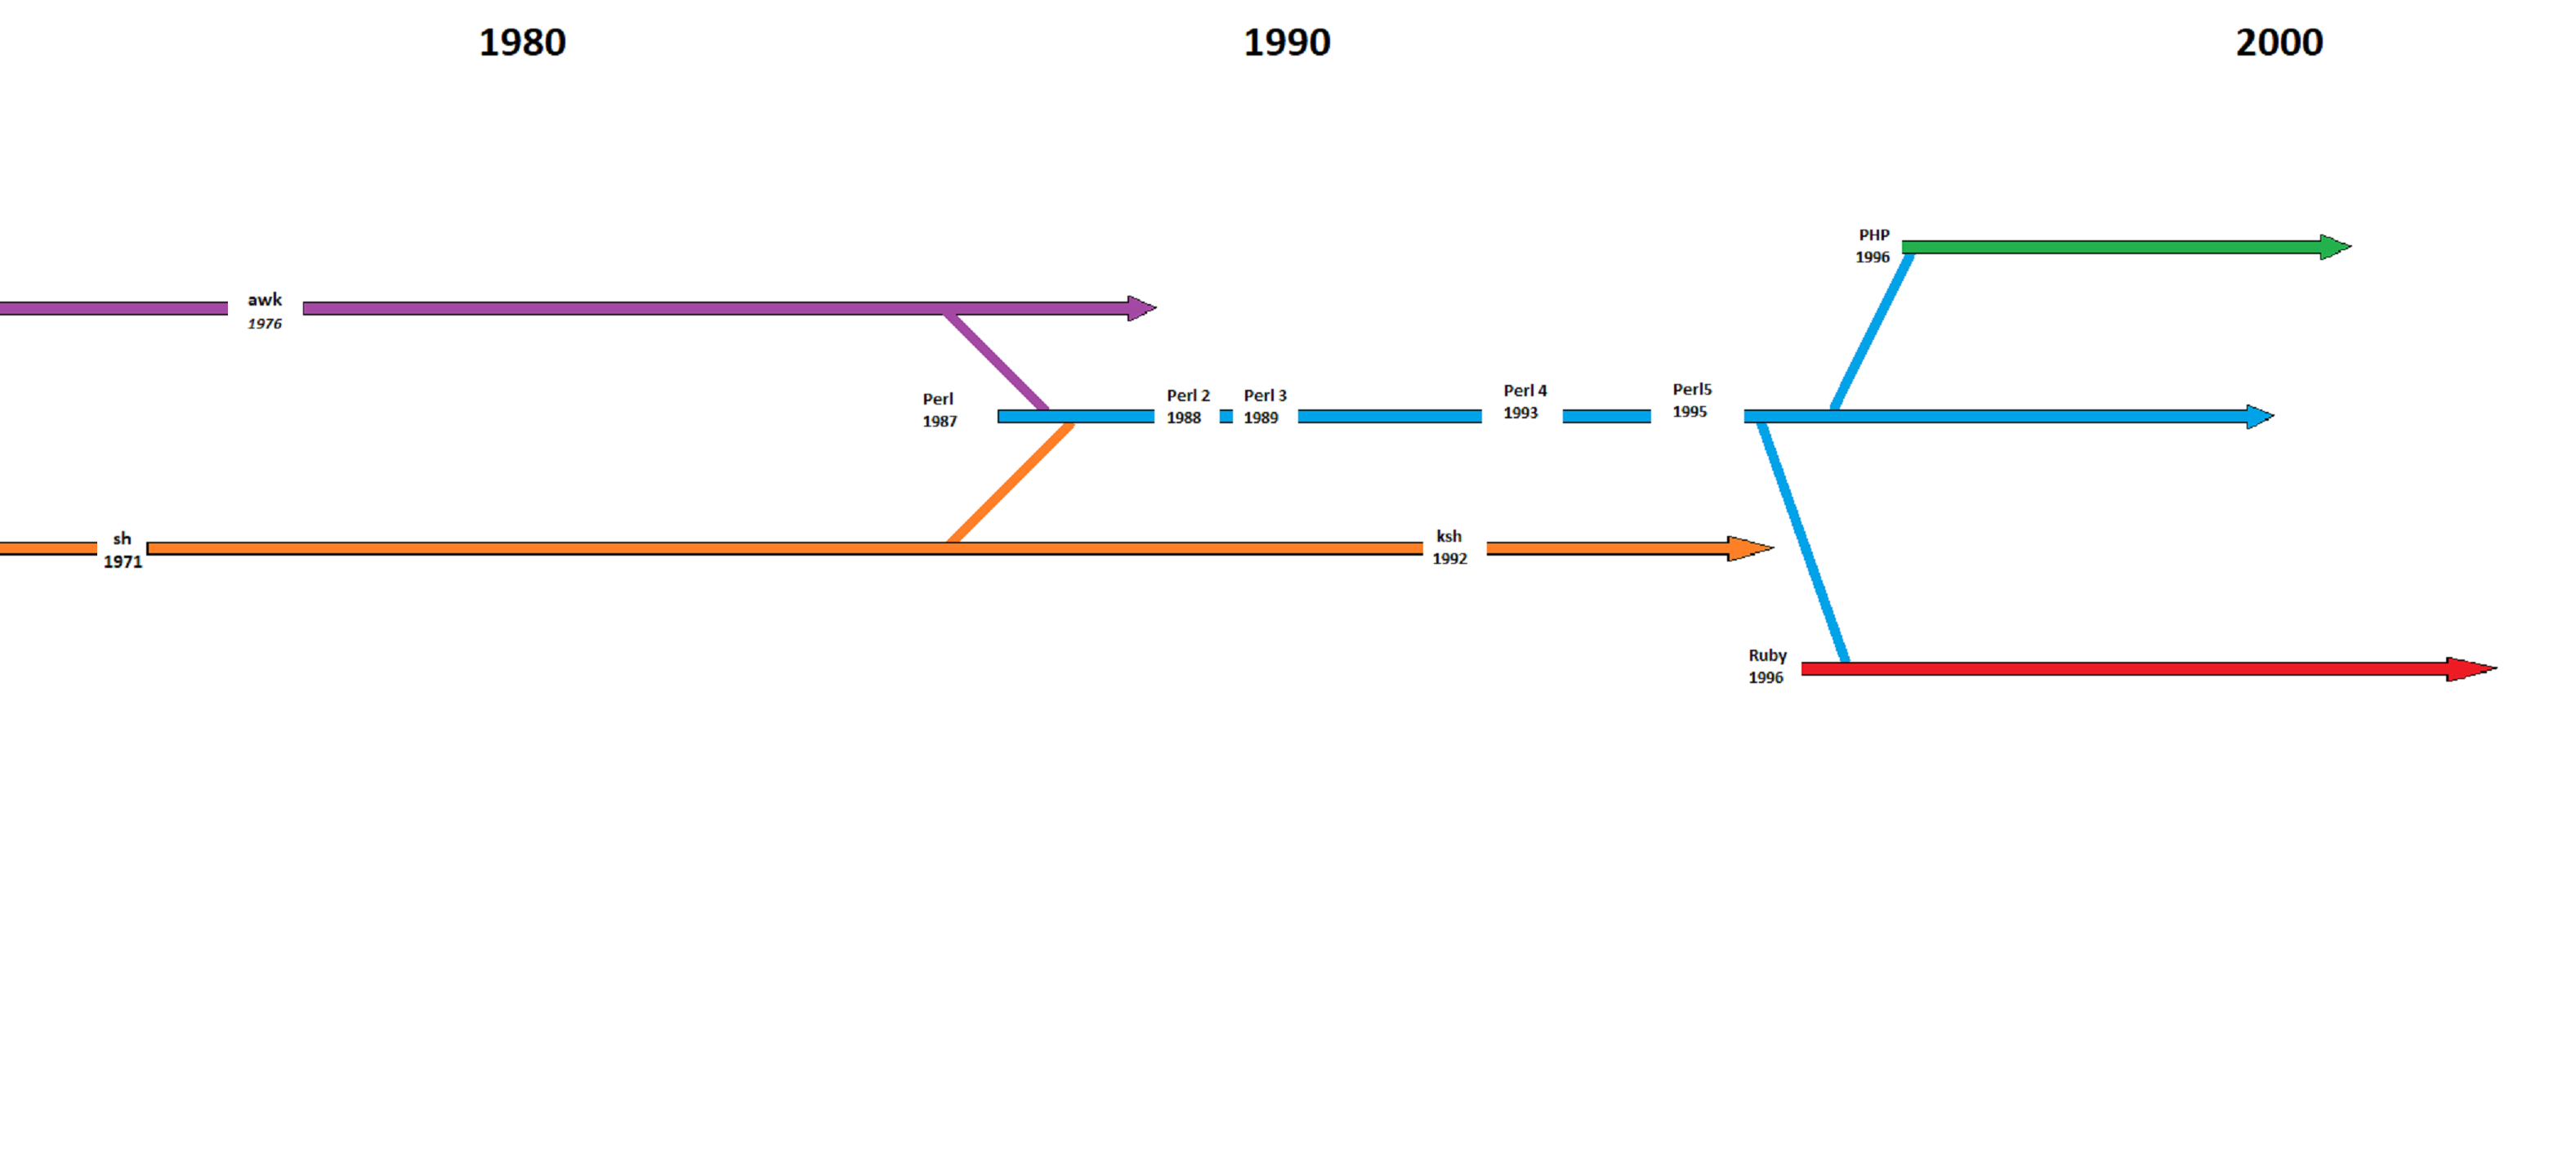
\includegraphics[scale=0.25,angle=90]{drvoRazvoja.png}
\caption{Drvo razvoja}
\end{figure}
Iako su početci Perla mnogo predhodili internetu konstantnim evoluiranjem nikada nije prestao da bude relevantan.Verzija 5.004 donosi nam modul koji obezbedjuje API za pisanje web aplikacija. Krajem devedesetih nazivan je lepkom koji odrzava internet. Nece nas iznenaditi da u razvojnom stablu programskih jezika zauzima mesto predaka PHP.\\
Sredinom poslednje decenije dvadesetog veka Yukihiro Matsumoto želi da objedini moć tekstualnog procesiranja Perla sa Pythonom. 1993 objavljuje programski jezik Ruby.



\section{Osnovna namena, svrhe i mogucnosti}

Glavna snaga Perla ogleda se u radu sa regularnim izrazima. Tri glavne operacije su uparivanje(eng. matching),zamena uparenog string drugim i prevođenje koje menja karaktere iz liste sa odgovarajućim karakterima iz liste zamena\cite{id}, a ono sto ga razlikuje od drugih je to što su regex izrazi "građani prvog reda"\cite{prviRed}. Postoje brojne modifikacije regex operatora koje olakšavaju korišćenje i pružaju veliki broj opcija programeru. Na usluzi programeru nalaze se i četiri promenljive u kojima se cuvaju rezulatati poslednjeg uparivanja. Imamo pristup sledećim informacijama:da li je došlo do uparivanja,upareni string,string pre uparenog i string posle\cite{friedl2006mastering}. Kada drugi programski jezici predstavljaju svoje mogućnosti vezane za parsiranje texta i regularne izrade uglavnom to čine poredeći se upravo sa Perlom.\\
Bezbednost je jedna od najznačajnih komponenti svakog programa, od naglog razvoja mreznog programiranja bezbednost eksponencijalno dobija na značaju. Već smo pomenuli da Perl pronalazimo kao bekend(eng {\em back end}) skripting jezik u mreznom programiranju. Veliki razlog za to je tejnted mod rada(eng. {\em Tainted}). Kada Perl operiše u ovom režimu rada svakom podatku koji dolazi od korisnika ili iz okruženja pokretanja dodaje se malo meta podataka koji ukazuje da ti podatci mogu potencijalno biti problematični. U svakom trenutku u programu se moze proveriti poreklo podataka i izdvojiti "siguran" deo istog\cite{modern}.\\
Kao odgovor na sve ceću potraznju objektno orijentisanih jezika Perl nudi biblioteku Moose. Moose nudi osnovne mogucnosti kao sto su pravljenje klasa, metoda, atributa ali i podrzava koncepte kao sto su nasledjivanje i preopterećivanje metoda. 

\pagebreak






\bibliography{bibliography.bib}
\bibliographystyle{abbrv}
\end{document}

